\documentclass{beamer}

%\usefonttheme{professionalfonts} % using non standard fonts for beamer
%\usefonttheme{serif} % default family is serif
%\usepackage{fontspec}
%\setmainfont{Lato}

\usepackage[russian]{babel}
\usepackage[backend=biber, style=gost-numeric]{biblatex} 
\addbibresource{javatime.bib}

\usepackage{graphicx}
\usepackage{listings}
\usepackage{color}

\definecolor{codegreen}{HTML}{0e7d17}
\definecolor{codegray}{HTML}{8c8c8c}

\lstset{ %
%  backgroundcolor=\color{white},   % choose the background color
  basicstyle=\footnotesize,        % size of fonts used for the code
  breaklines=true,                 % automatic line breaking only at whitespace
  captionpos=b,                    % sets the caption-position to bottom
  commentstyle=\color{codegray},    % comment style
  escapeinside={\%*}{*)},          % if you want to add LaTeX within your code
  keywordstyle=\color{blue},       % keyword style
  stringstyle=\color{codegreen},     % string literal style
  frame=single,
}

% 0e7d17

% Theme choice:
\usetheme{metropolis} 
\setsansfont{Lato}
\setmonofont{FreeMono}
%\usepackage[sfdefault]{biolinum}

%\usetheme{CambridgeUS}

% Title page details: 
\title{Введение в GraphQL} 
\author{Андрей Накин}
\date{\today}

\begin{document}

% Title page frame
\begin{frame}
    \titlepage 
\end{frame}

% Remove logo from the next slides
%\logo{}


% Outline frame
\begin{frame}{Outline}
    \tableofcontents
\end{frame}

\begin{frame}{{\tt java.time}}

Пакет {\tt java.time} (первый выпуск в 2014~году):

\begin{itemize}
    \item Более удобное API.
    \item Иммутабельные классы.
    \item Новые типы для неполной спецификации времени ({\tt LocalTime}, {\tt LocalDate} и~др.).
    \item API для работы с временными промежутками ({\tt Duration}, {\tt Period}).
    \item Управление системным временем ({\tt Clock}, удобно в~тестах).
    \item Удалена поддержка Юлианского календаря~:(
\end{itemize}

\end{frame}

\section{{\tt ZonedDateTime}}

\begin{frame}[fragile]{{\tt ZonedDateTime} / Исторические изменения}

{\tt ZonedDateTime} учитывает исторические изменения характеристик временной зоны:
\bigskip

\begin{lstlisting}[language=java]
ZoneId tz = ZoneId.of("Europe/Moscow");
ZonedDateTime ztd = ZonedDateTime.of(
  LocalDateTime.parse("2022-01-01T01:00:00"), tz);

out.println(ztd.withYear(2011).getOffset()); // +03:00
out.println(ztd.withYear(2014).getOffset()); // +04:00
out.println(ztd.withYear(2015).getOffset()); // +03:00
\end{lstlisting}

Временные зоны и часовые пояса меняются довольно часто, например в РФ последнее изменение было в~2020~году \cite{dst_news}.

\end{frame}

\begin{frame}[fragile]{{\tt ZonedDateTime} / Исторические изменения}

  Для своей работы {\tt ZonedDateTime} использует базу данных временных зон --- Time Zone Database или {\tt tzdata} \cite{tzdata}, для которой регулярно выходят обновления.

    \begin{alertblock}{Важное следствие}
     	Чтобы ваше приложение, использующее {\tt ZonedDateTime}, работало правильно, необходимо обеспечить обновление этой базы!
    \end{alertblock}

\end{frame}

\begin{frame}[fragile]{{\tt ZonedDateTime} / Исторические изменения}

  Как обновляется информация о временных зонах?

  \begin{block}{Oracle JDK}
  	База данных временных зон включена в дистрибутив. Узнать версию базы можно по таблице соответствий \cite{oracle_tzdata}. 
  	
  	Для обновления базы данных требуется обновление версии JDK. Также можно обновить существующую версию при помощи утилиты {\tt tzupdater} \cite{tzupdater}.
  \end{block}

\end{frame}

\begin{frame}{Пользовательский {\tt ZoneRulesProvider}}
    Похоже, тема пользовательского {\tt ZoneRulesProvider} не особо популярна:
    
    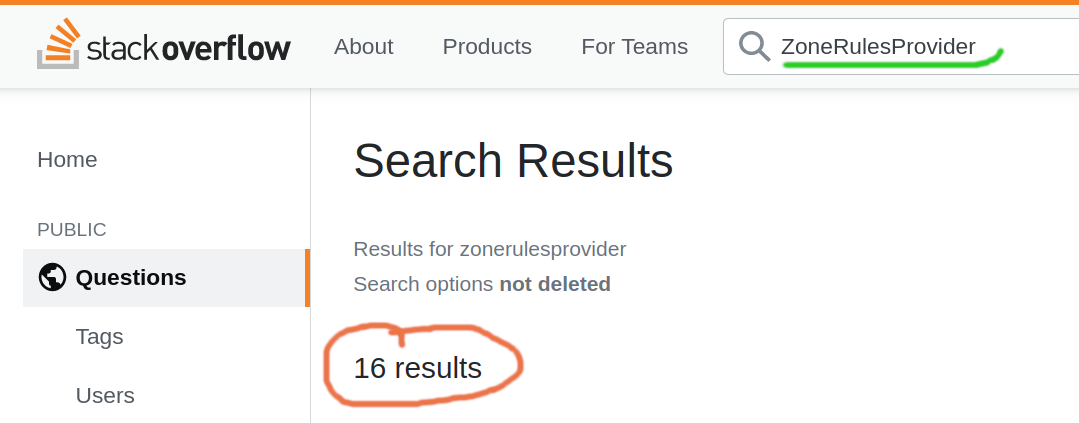
\includegraphics{png/so-results}
\end{frame}
  
% Lists frame
\section{Списки в Beamer}
\begin{frame}{Списки в Beamer}

Это неупорядоченный список:
\begin{itemize}
    \item Пункт 1
    \item Пункт 2
    \item Пункт 3
\end{itemize}

and this is an ordered list:
\begin{enumerate}
    \item Item 1
    \item Item 2
    \item Item 3
\end{enumerate}

\end{frame}


\begin{frame}[fragile]{API сотрудников}
\begin{verbatim}
curl https://my-api.io/employees/emp-1
\end{verbatim}

Ответ:

\begin{verbatim}
{
  "id":            "emp-1",
  "given":         "Илья",
  "patronym":      "Ильич",
  "family":        "Обломов",
  "department_id": "dep-1",
  "photo":         "/9j/4AAQSkZJRgABAQAA..."
}
 
\end{verbatim}

\end{frame}

\begin{frame}[fragile]{API отделов}
\begin{verbatim}
curl https://my-api.io/departments/dep-1
\end{verbatim}

Ответ:

\begin{verbatim}
{
  "id":   "dep-1",
  "name": "Производственный"
}
\end{verbatim}

\end{frame}

% Blocks frame
\section{Blocks in Beamer}
\begin{frame}{Blocks in Beamer}
    \begin{block}{Standard Block}
        This is a standard block.
    \end{block}
    \begin{alertblock}{Alert Message}
        This block presents alert message.
    \end{alertblock}
    \begin{exampleblock}{An example of typesetting tool}
        Example: MS Word, \LaTeX{}
    \end{exampleblock}
\end{frame} 

\begin{frame}{Библиография}

\printbibliography

\end{frame}

\end{document}
